\section{Crowd Counting Model}
\subsection{CCTrans}
CCTrans aims to simplify and improve the performance of crowd counting models by leveraging the global modeling capability of Transformers. Traditional CNN-based methods often struggle with complex scenes due to limited receptive fields and insufficient contextual awareness. In contrast, CCTrans uses a pure Transformer-based backbone to better capture both local and global information in crowd images. The overall architecture is illustrated in Figure ~\ref{fig:cctrans_pipeline}. It mainly includes three parts:
\begin{figure}[H]
    \centering
    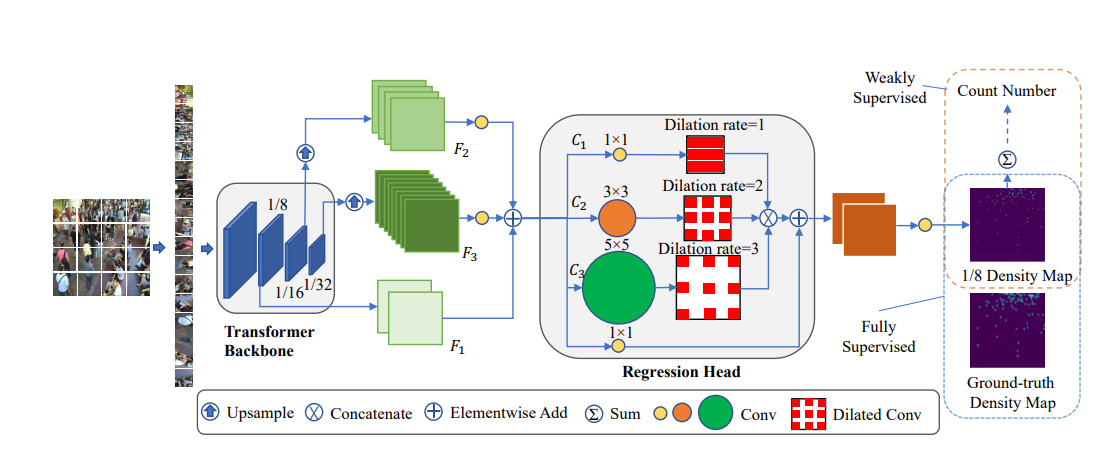
\includegraphics[width=1\linewidth]{related-work/image/pipline.png}
    \caption{The pipeline of CCTrans. It uses a pyramid Transformer backbone for feature extraction, followed by pyramid feature aggregation and a multi-scale regression head. The model supports both fully-supervised (density map) and weakly-supervised (count regression) settings.}
    \label{fig:cctrans_pipeline}
\end{figure}
\textbf{2D Image to 1D Sequence}\\

Given an input image \( I \in \mathbb{R}^{H \times W \times 3} \), where \( H \) and \( W \) are the image height and width respectively, and 3 represents the RGB color channels, we first divide the image into non-overlapping square patches of size \( K \times K \).

\begin{itemize}
    \item The total number of patches is:
    \[
    N = \frac{H \times W}{K^2}
    \]
    
    \item Each patch has a shape \( K \times K \times 3 \) and is flattened into a vector of dimension:
    \[
    D = K \times K \times 3
    \]
    
    \item This results in a patch sequence:
    \[
    x \in \mathbb{R}^{N \times D}
    \]
    
    \item To prepare the sequence for the Transformer, we apply a learnable linear projection:
    \[
    f: x_i \mapsto e_i \in \mathbb{R}^{D'}
    \quad \text{for } i = 1, \dots, N
    \]
    where \( D' \) is the desired embedding dimension.

    \item The final embedded sequence is:
    \[
    e \in \mathbb{R}^{N \times D'}
    \]
\end{itemize}

This embedding process transforms the spatial and channel-wise information of each patch into a vector representation suitable for input into a Transformer encoder.\\
\textbf{Pyramid Vision Transformer (PVT)}\\
The Twins architecture \cite{chu2021twins} is a pyramid-style Transformer backbone that alternates between local and global self-attention mechanisms. By incorporating both local and global receptive fields, it captures short- and long-range dependencies effectively, resulting in strong performance across a variety of benchmarks.

Twins introduces a module called \textbf{Spatially Separable Self-Attention (SSSA)} to reduce computational cost. Specifically, the input sequence of the $l$-th layer, denoted as $Z_{l-1}$, is first reshaped into a 2D feature map. The attention computation is then performed in two stages:

\begin{itemize}
    \item \textbf{Locally-grouped Self-Attention (LSA)}: the feature map is evenly divided into $k_1 \times k_2$ non-overlapping sub-windows. Self-attention is computed independently within each sub-window, allowing for efficient local feature extraction.

    \item \textbf{Global Subsampled Attention (GSA)}: each sub-window generates a representative feature using a convolution operation. These representatives summarize the key information of their respective regions. Self-attention is then computed across all representatives, enabling communication between spatially distant regions and capturing global context.
\end{itemize}

The Swin Transformer, introduced by Liu et al.~\cite{liu2021swin}, builds upon the hierarchical Transformer idea by introducing a localized self-attention mechanism that scales efficiently with image size. Rather than applying self-attention globally, it performs attention within non-overlapping local windows. This results in linear computational complexity with respect to image size, a significant improvement over the quadratic cost of global attention.

To enable interaction across different windows, the Swin Transformer introduces a shifted window strategy. Specifically, in alternating layers, the window partitioning is shifted by a fixed number of pixels (typically half the window size), which enables neighboring patches from adjacent windows to be grouped together. This mechanism allows for cross-window connections without significantly increasing computation, effectively capturing both local and global context.

Follow the structure of image image \ref{fig:swin}, Each Swin Transformer block contains two successive attention layers: a regular window-based multi-head self-attention (W-MSA) and a shifted window multi-head self-attention (SW-MSA). These are followed by multilayer perceptrons (MLPs) with residual connections and layer normalization. Between stages, patch merging is performed by concatenating neighboring tokens and applying a linear transformation to reduce spatial resolution while increasing channel dimensions, supporting hierarchical representation learning.
\begin{align}
\hat{z}^{l} &= \text{W-MSA}\left(\text{LN}\left(z^{l-1}\right)\right) + z^{l-1}, \\
z^{l} &= \text{MLP}\left(\text{LN}\left(\hat{z}^{l}\right)\right) + \hat{z}^{l}, \\
\hat{z}^{l+1} &= \text{SW-MSA}\left(\text{LN}\left(z^{l}\right)\right) + z^{l}, \\
z^{l+1} &= \text{MLP}\left(\text{LN}\left(\hat{z}^{l+1}\right)\right) + \hat{z}^{l+1},
\end{align}

where $\hat{z}^{l}$ and $z^{l}$ denote the output features of the (S)W-MSA module and the MLP module for block $l$, respectively. \cite{liu2021swin}

The Swin Transformer has been shown to perform strongly across a wide range of computer vision tasks, including image classification, object detection, and semantic segmentation, and has become a foundational architecture for vision backbones.

\begin{figure}[h]
    \centering
    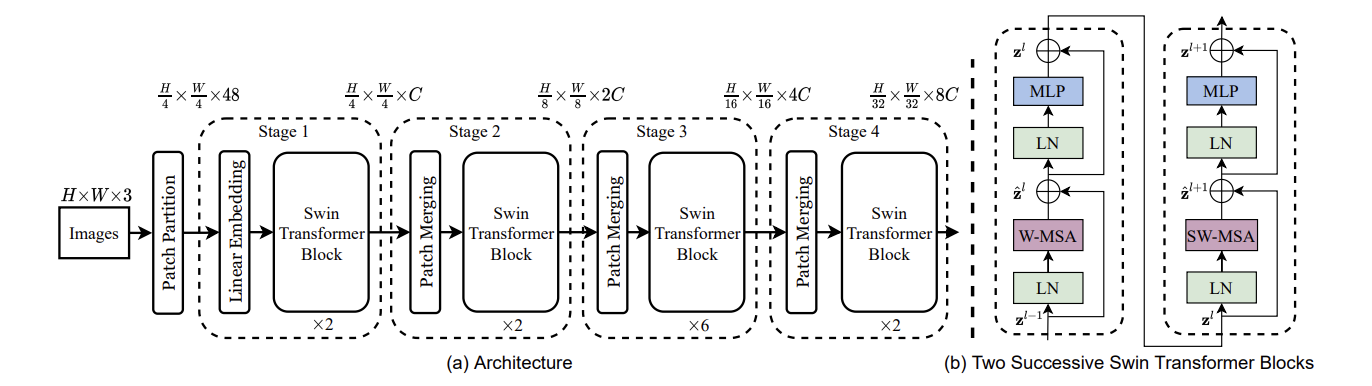
\includegraphics[width=0.75\linewidth]{SwinTrans.png}
    \caption{Swin Transformer, \cite{liu2021swin}}
    \label{fig:swin}
\end{figure}

Here, LN denotes Layer Normalization, MLP refers to a multi-layer perceptron, and each residual connection (addition) helps preserve gradient flow and improve model stability. The interleaving of local and global attention enables the model to effectively extract both fine-grained details and global semantics.

\textbf{Pyramid Feature Aggregation (PFA)}\\
Although the Transformer backbone can capture both local and global contexts, the feature maps produced by deeper layers often lose fine spatial details, which are crucial for tasks requiring precise localization such as crowd counting. High-level features tend to be more abstract and lack clear boundary information, making it difficult to accurately identify object locations.

To address this issue, the Pyramid Feature Aggregation (PFA) module is designed to fuse multi-scale features from different stages of the backbone. The feature maps from each stage, which contain complementary information—low-level layers providing rich spatial details and high-level layers offering strong semantic context—are first upsampled to a common spatial resolution, typically \( \frac{1}{8} \) of the input image size. Since these feature maps often differ in channel dimensions, a projection operation (commonly a \(1 \times 1\) convolution or linear layer) is applied to unify their channel numbers. This allows for efficient element-wise fusion through addition or concatenation.

By aggregating features across scales, PFA enhances the model's ability to retain detailed spatial information while leveraging high-level semantic cues, ultimately improving performance on dense prediction tasks.
\textbf{Multi-scale Dilated Convolution (MDC) Head}\\
After the Pyramid Feature Aggregation (PFA) block, the fused feature map contains multi-scale information from different stages of the backbone. To effectively utilize this rich information for accurate density map regression, a multi-scale receptive field module is employed in the regression head. Inspired by the Multi-scale Dilated Convolution (MDC) design \cite{li2018csrnet, chen2018encoder}, the regression head processes the aggregated features through parallel convolutional layers with different kernel sizes and dilation rates.

Specifically, three parallel columns are used, each consisting of a standard convolution followed by a dilated convolution (as show in Fig~\ref{fig:dialted}). The kernel sizes and dilation rates are carefully chosen to cover various receptive fields: a small kernel (e.g., 1×1) captures fine local details, a medium kernel (e.g., 3×3) covers local neighborhoods, and a larger kernel (e.g., 5×5 or dilated 3×3) captures broader context. Each convolution layer is followed by batch normalization and ReLU activation to enhance training stability and non-linearity.

The outputs of these parallel convolutions are concatenated and combined with a shortcut connection to preserve original features and enrich multi-scale representations. Finally, a 1×1 convolutional layer is applied to regress the final density map. This design balances model complexity and receptive field diversity, improving crowd counting accuracy while avoiding issues like the gridding effect common in stacked dilated convolutions.
\begin{figure}[H]
    \centering 
    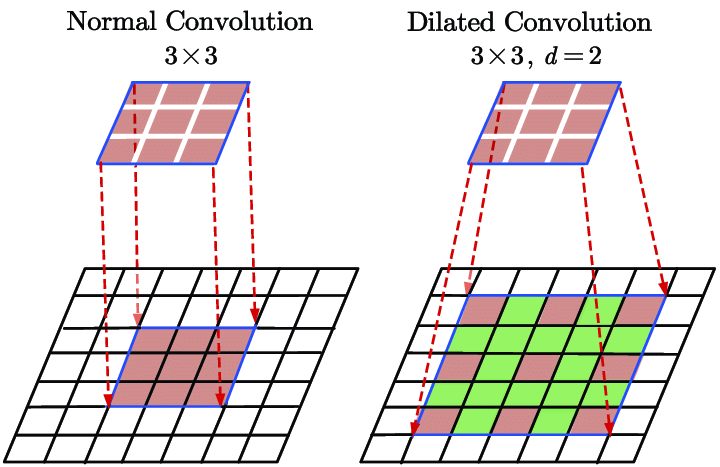
\includegraphics[width=8cm]{related-work/image/dilated.png} 
    \caption{Compare Normal Conv and Dilated Conv} 
    \label{fig:dialted}
\end{figure}
\textbf{Loss Function Design}
\begin{itemize}
    \item \textbf{Fully - supervised}\\
    The training process is guided by a composite loss function adapted from DM-Count~\cite{wang2020distribution}, which combines global count error and density map distribution alignment. The overall loss is defined as:
    
    \begin{equation}
    \mathcal{L}_d = \mathcal{L}_1(P, G) + \lambda_1 \mathcal{L}_{OT} + \lambda_2 \mathcal{L}_2(D, D_0)
    \end{equation}

    where $\mathcal{L}_1(P, G)$ penalizes the difference between the predicted count $P$ and ground-truth count $G$, $\mathcal{L}_{OT}$ is the Optimal Transport loss to align spatial distributions, and $\mathcal{L}_2(D, D_0)$ is the mean squared error between the predicted map $D$ and the smoothed ground-truth $D_0$ (obtained via adaptive Gaussian kernels~\cite{li2018CSRNet}).

    This design addresses the limitations of total variation (TV) loss in sparse regions and provides stronger supervision on local structures. Following~\cite{wang2020distribution}, $\lambda_1$ is set to 0.01 and $\lambda_2$ is treated as a tunable parameter.
    \item \textbf{Weakly - supervised}
The loss function for the weakly-supervised setting is defined using Smooth L1 loss to provide robust training signals. As the number of people varies significantly across different images, using standard L1 loss can be sensitive to outliers. Smooth L1 mitigates this issue by behaving like L2 loss when the error is small and L1 when the error is large, thus offering a balanced and stable optimization target:
\begin{equation}
\mathcal{L}_c = \text{SmoothL1}(D, D_0)
\end{equation}
This design ensures that the model can learn effectively from weak annotations, without being overly influenced by extreme variations in crowd density.
\end{itemize}

\subsection{FFNet}
The Fuss-Free Network (FFNet) \cite{gao2025effectiveness} represents a paradigm shift towards simplified yet effective crowd counting models. Unlike existing complex architectures that achieve high performance through increased structural complexity, FFNet demonstrates that excellent crowd counting results can be obtained using a streamlined design consisting of only two primary components: a backbone network and a multi-scale feature fusion structure.
\subsubsection{Overall Architecture Design}
\begin{figure}[ht]
    \centering
    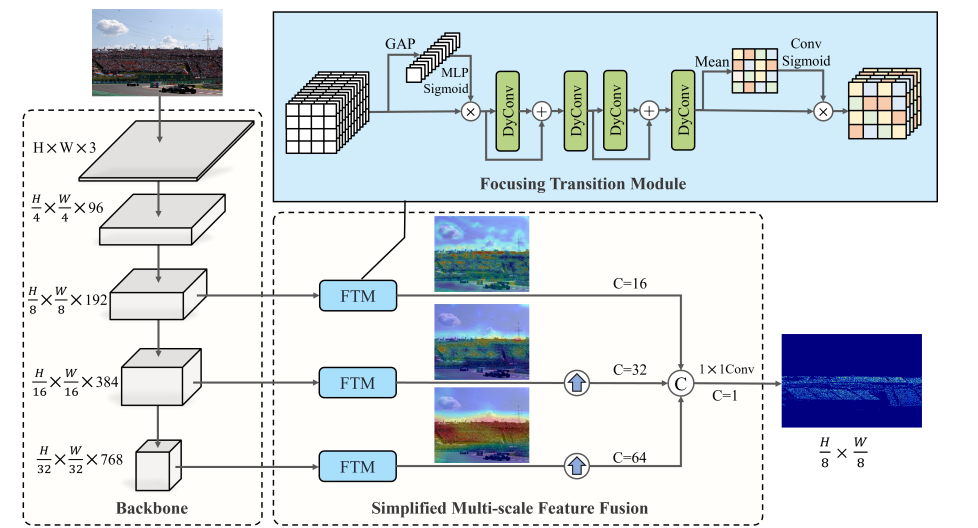
\includegraphics[width=1\linewidth]{related-work/image/ffnet_architecture.png}
    \caption{The network architecture of FFNet. H, W, C denote the height, width, and number of channels of the features, respectively. And the circles with “×”, “+”, and “C” represent element-wise multiplication, element-wise addition, and channel concatenation operations, respectively \cite{gao2025effectiveness}}
    \label{fig:ffnet_architecture}
\end{figure}
FFNet's architecture philosophy centers on simplicity and efficiency while maintaining competitive performance. The model comprises a ConvNeXt-Tiny \cite{liu2022convnet} backbone for feature extraction and a simplified multi-scale feature fusion module that processes features at three different scales. This design deliberately avoids the intricate multi-decoder blocks, sophisticated fusion headers, and complex transformer-based encoder-decoder structures commonly found in contemporary crowd counting models.\\
The network extracts features from three different stages of the backbone $(S_{1}, S_{2}, S_{3})$, where each stage captures information at varying spatial resolutions and semantic levels. These multi-scale features are then processed through individual focus transition modules before being fused to generate the final density map.
\subsubsection{Feature Extraction Backbone}
ConvNeXt-Tiny serves as the feature extraction backbone, chosen for its balance of simplicity and effectiveness. This architecture builds upon the foundation of ResNet \cite{he2016deep} while incorporating modern design principles inspired by Vision Transformers \cite{dosovitskiy2020image} and ResNeXt \cite{xie2017aggregated}. Key architectural improvements include adjusted stage compute ratios, inverted bottleneck structures, large kernel sizes, and the substitution of ReLU with GELU activation functions. \\
The backbone preserves the strong spatial processing capabilities of CNNs for local feature extraction while significantly improving global information comprehension and utilization. To address the varying object sizes inherent in crowd counting tasks, features are extracted from diverse stages of ConvNeXt-Tiny, enabling the model to capture hierarchical features at different resolutions from each processing stage.
\subsubsection{Multi-Scale Feature Fusion Strategy}
The multi-scale feature fusion component addresses the fundamental challenge of scale and density variations within crowd images. Three fusion strategies were evaluated: concatenate fusion, addition fusion, and stepwise addition fusion.\\
The adopted concatenate fusion strategy directly applies transposed convolution to features $S_{2}$ and $S_{3}$ for upsampling to match the spatial dimensions of $S_{1}$, followed by channel concatenation. This approach was selected over alternative fusion methods due to its superior performance in experimental validation. Transposed convolution operations are specifically chosen over interpolation methods for their learning capability, flexibility, spatial accuracy, and ability to handle irregular patterns in complex crowd distribution scenarios.
\subsubsection{Focus Transition Module (FTM)}
The Focus Transition Module represents a critical innovation in FFNet's architecture, designed to bridge the gap between general-purpose backbone features and crowd-specific representations. Since the backbone network was originally designed for classification tasks, its output features contain general semantic information that differs from the specialized features required for crowd counting applications.\\
FTM comprises three main components working in sequence:
\begin{itemize}
    \item Channel Attention Mechanism: Captures interdependencies among different feature map channels extracted from the backbone network. This mechanism assigns importance weights to each channel based on their significance, enabling the network to focus on relevant crowd-related features while suppressing less informative channels.
    \item Dynamic Convolution-Based Feature Transformation: The core component utilizes dynamic convolution as an alternative to conventional convolution operations, effectively enhancing the model's representational power without increasing network depth or width. Dynamic convolution dynamically combines multiple parallel convolution kernels based on attention weights determined by input data, generating convolution kernel weights during runtime for adaptive feature extraction across various dimensions including input channels, output channels, kernel size, and kernel count.
    \item Spatial Attention Mechanism: Captures spatial interdependencies within feature maps by assigning weights to different spatial locations, allowing the network to focus on relevant spatial regions while suppressing irrelevant or noisy areas.
\end{itemize}
The mathematical formulation of FTM operations follows:
\begin{center}
    C (F) = $ \sigma $ (MLP (AvgPool (F)) $ \odot $ F, \\ P (C) = Y [Y (Y (Y (C) + C) + (Y (C) + C))], \\ S (P) = $ \sigma $ (Conv ( $ \overline {P} $)) $ \odot $
\end{center}
where F represents the input, $C(.)$ denotes channel feature weight optimization, $Y(.)$ represents dynamic convolution operations, $P(.)$ is the output after stacked dynamic convolutions, and $S(.) $performs spatial feature weight optimization.\\
The FTM design incorporates residual connections throughout the entire process to enhance gradient flow and facilitate learning of intricate relationships. Additionally, the module implicitly achieves feature dimensionality reduction while preserving key information integrity, thereby reducing computational complexity.
\subsubsection{Network Output and Density Map Generation}
The final stage of FFNet processes the concatenated multi-scale features through a 1×1 convolution layer to merge features into a single channel, producing the final crowd density map. This density map provides pixel-level crowd distribution estimates, from which the total crowd count is obtained through spatial integration.\\
The streamlined architecture of FFNet demonstrates that effective crowd counting can be achieved without excessive structural complexity, making it particularly suitable for deployment in resource-constrained environments while maintaining competitive performance with state-of-the-art methods.

\subsection{Loss Function in Crowd Counting}

The loss function employed in the Fuss-Free Network (FFNet) for crowd counting, as detailed in the referenced paper \cite{gao2025effectiveness}, is a composite loss derived from the Distribution Matching for Crowd Counting (DM-Count) framework \cite{wang2020distribution}. This loss function is pivotal in optimizing the FFNet model, ensuring accurate crowd density estimation by aligning the predicted density maps with ground truth annotations. The total loss comprises three components: count loss, optimal transport (OT) loss, and variation loss. Each component addresses specific aspects of the crowd counting task, balancing accuracy, distribution alignment, and smoothness in the predicted density maps. Below, we provide a detailed explanation of each component, their mathematical formulations, and their significance in the context of FFNet's performance.

\subsubsection{Count Loss}
The count loss, denoted as $\mathcal{L}_c$, quantifies the discrepancy between the total number of individuals predicted by the model and the actual number labeled in the ground truth. This loss ensures that the model accurately estimates the crowd count, which is the primary objective of crowd counting tasks. It is defined as:

\begin{equation}
\mathcal{L}_c(\mathbf{z}, \hat{\mathbf{z}}) = \|\mathbf{z}\|_1 - \|\hat{\mathbf{z}}\|_1,
\end{equation}

where $\mathbf{z}$ represents the vectorized binary map of dot annotations (ground truth), $\hat{\mathbf{z}}$ is the vectorized predicted density map, and $\|\cdot\|_1$ denotes the L1 norm. The count loss directly penalizes errors in the total crowd count, promoting convergence towards accurate numerical predictions. In FFNet, this loss is critical for ensuring that the simplified model structure, consisting of a ConvNeXt-Tiny backbone and a multi-scale feature fusion module, maintains high counting accuracy despite its reduced complexity.

\subsubsection{Optimal Transport Loss}
The optimal transport (OT) loss, $\mathcal{L}_{ot}$, is employed to align the predicted density map with the ground truth distribution, addressing the challenge of misaligned data distributions in crowd counting. This loss leverages the principles of optimal transport to measure the difference between two probability distributions, encouraging the model to produce density maps that closely match the true distribution of crowd annotations. The OT loss is particularly effective in handling scenarios with varying crowd densities and occlusions, which are common in crowd counting datasets. It is defined as:

\begin{equation}
\mathcal{L}_{ot}(\hat{\mathbf{z}}) = \left\langle \frac{\beta^*}{\|\hat{\mathbf{z}}\|_1} - \frac{\langle \beta^*, \hat{\mathbf{z}} \rangle}{\|\hat{\mathbf{z}}\|_1^2}, \hat{\mathbf{z}} \right\rangle,
\end{equation}

where $\beta^*$ represents the dual variables computed using the Sinkhorn algorithm \cite{peyre2019computational}, and $\langle \cdot, \cdot \rangle$ denotes the dot product. The Sinkhorn algorithm iteratively optimizes the transportation plan from the predicted density map to the ground truth, ensuring that the model learns a probability density that aligns with the actual crowd distribution. In the context of FFNet, the OT loss enhances the model's ability to capture complex crowd patterns, compensating for the simplified architecture by improving the quality of the generated density maps.

\subsubsection{Variation Loss}
The variation loss, $\mathcal{L}_v$, is designed to enhance the smoothness of the predicted density map by minimizing intensity or grayscale variations between adjacent pixels. This loss is particularly important for reducing noise and ensuring that the density map is visually coherent, especially in regions with varying crowd densities. It is defined as:

\begin{equation}
\mathcal{L}_v(\mathbf{z}, \hat{\mathbf{z}}) = \|\mathbf{z}\|_1 \cdot \|\mathbf{z} - \hat{\mathbf{z}}\|_1,
\end{equation}

where the L1 norm is used to measure the difference between the ground truth and predicted density maps, weighted by the actual crowd count $\|\mathbf{z}\|_1$. This weighting factor balances the contribution of the variation loss across regions with different crowd densities, ensuring that the model prioritizes accuracy in high-density areas while maintaining smoothness. For FFNet, the variation loss complements the simplified multi-scale feature fusion strategy by refining the density map output, mitigating potential artifacts introduced by the concatenation operation.

\subsubsection{Total Loss}
The total loss function for FFNet is a weighted sum of the three components, defined as:

\begin{equation}
\mathcal{L}_{all} = \mathcal{L}_c + \lambda_1 \mathcal{L}_{ot} + \lambda_2 \mathcal{L}_v,
\end{equation}

where $\lambda_1 = 0.1$ and $\lambda_2 = 0.01$ are empirically determined weighting factors that balance the contributions of the OT and variation losses relative to the count loss. This composite loss ensures that FFNet optimizes for both numerical accuracy (via count loss), distribution alignment (via OT loss), and spatial smoothness (via variation loss). The careful calibration of these weights allows FFNet to achieve state-of-the-art performance on datasets such as UCF\_CC\_50, ShanghaiTech Part A, and ShanghaiTech Part B, despite its simplified structure.

\subsubsection{Significance in FFNet}
The adoption of the DM-Count loss function in FFNet is a strategic choice that enhances the model's effectiveness within the constraints of a simplified architecture. The count loss ensures numerical accuracy, which is critical for practical applications such as urban management and public safety monitoring. The OT loss addresses the challenge of varying crowd densities and occlusions, enabling FFNet to generalize across diverse scenarios. The variation loss refines the density map, making it robust to noise and suitable for real-time applications on resource-constrained systems like Deep Stream. Experimental results demonstrate that FFNet, with this loss function, achieves a Mean Absolute Error (MAE) of 161.4 on UCF\_CC\_50, 48.3 on ShanghaiTech Part A, and 6.1 on ShanghaiTech Part B, outperforming or matching complex models while maintaining lower computational complexity (29.02M parameters and 23.67G FLOPS with ConvNeXt-Tiny backbone).

\subsubsection{Integration with Deep Stream System}
In the context of the Deep Stream system, the loss function's efficiency is crucial for real-time crowd counting. The simplified structure of FFNet, combined with the DM-Count loss, allows for rapid convergence during training and efficient inference on hardware with limited resources, such as the 16-GB RTX 4080 used in the experiments. The OT loss, with its Sinkhorn algorithm, is computationally efficient due to its iterative optimization approach, making it suitable for deployment in Deep Stream environments where low latency is essential. Furthermore, the variation loss ensures that the density maps are smooth and interpretable, facilitating integration with visualization tools in Deep Stream for real-time crowd monitoring.